\documentclass[11pt]{article}  
\usepackage[margin=1in]{geometry}
\parindent=0in
\parskip=8pt
\usepackage{fancyhdr,amssymb,amsmath, graphicx, listings,float,subfig,enumerate,epstopdf,color,multirow,setspace,bm,textcomp}
\usepackage[usenames,dvipsnames]{xcolor}
\usepackage{hyperref}
\usepackage{graphicx}
\usepackage{tikz}
\graphicspath{{./Images}}

\pagestyle{fancy}


\begin{document} 

\lhead{Assignment \# 1}
\chead{Robert Denim Horton}
\rhead{\today}

\begin{center}\begin{Large}
CS 4720/5720 Design and Analysis of Algorithms

Homework \#1

Student: (Robert Denim Horton)
\end{Large}
\end{center}


\section*{Answers to homework problems:}

\begin{enumerate}
\item One reason for graph theory’s power as a modeling tool is the fluidity with which one can formalize properties of large systems using the language of graphs, and then systematically explore their consequences. In this first set of questions, we will work through an example of this process using the concept of a pivotal node. First, recall from Chapter 2 that a shortest path between two nodes is a path of the minimum possible length. We say that a node X is pivotal for a pair of distinct nodes Y and Z if X lies on every shortest path between Y and Z (and X is not equal to either Y or Z).\\\\
For example, in the graph in Figure 2.13, node B is pivotal for two pairs: the pair consisting of A and C, and the pair consisting of A and D. (Notice that B is not pivotal for the pair consisting of D and E since there are two different shortest paths connecting D and E, one of which (using C and F) doesn’t pass through B. So B is not on every shortest path between D and E.) On the other hand, node D is not pivotal for any pairs.\\
\includegraphics[scale=0.9]{Figure_12_3}
	\begin{enumerate}[(a)]
		\item  Give an example of a graph in which every node is pivotal for at least one pair of nodes. Explain your answer.
		\item Give an example of a graph in which every node is pivotal for at least two different pairs of nodes. Explain your answer.
		\item  Give an example of a graph having at least four nodes in which there is a single
node X that is pivotal for every pair of nodes (not counting pairs that include X). Explain your answer.
	\end{enumerate}
\textcolor{gray}{
\begin{enumerate}[(a)]
\item  Given the formal definition of a pivotal node, a node can be difeind as such when the node of intrest exssits along every shortest possible path.  For example, given a graph with the set of nodes $S$ with defined nodes $\{A, \ B, \ C, \ D\}$.  The graph could be represented as;\\
\begin{center}
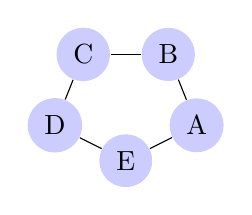
\begin{tikzpicture}[scale=0.9, auto=center, every node/.style={circle,fill=blue!20}] 
\node(A) at (1, -0.5) {A}; 
\node(B) at (0.6, 0.5) {B};
\node(C) at (-0.6, 0.5) {C}; 
\node(D) at (-1,-0.5) {D}; 
\node(E) at (0,-1) {E}; 
\draw(A) -- (B);
\draw(B) -- (C);
\draw(C) -- (D);
\draw(D) -- (E);
\draw(E) -- (A);
\end{tikzpicture}
\end{center}
As we can see in this diagram all the nodes are pivotal nodes.   Starting with the right most bottom node $A$, its pivotal nodes are $E$ and $B$, $B$ its pivotal nodes are $C$ and $A$, $C$ its pivotal nodes are $B$ and $D$,  and $D$ its pivotal nodes are $C$ and $E$.  Here we can see that every node that exsits has atleast one pair for each node that exists in the graph.\\
\item For a pivotal node to have two different pairs of nodes, we can define such nodes as nodes with pairs that are pivot nodes and that are simply make connection between  
\begin{center}
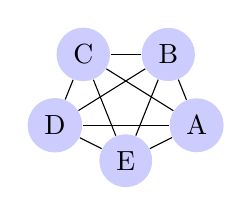
\begin{tikzpicture}[scale=0.9, auto=center, every node/.style={circle,fill=blue!20}] 
\node(A) at (1, -0.5) {A}; 
\node(B) at (0.6, 0.5) {B};
\node(C) at (-0.6, 0.5) {C}; 
\node(D) at (-1,-0.5) {D}; 
\node(E) at (0,-1) {E}; 
\draw(A) -- (B);
\draw(A) -- (C);
\draw(B) -- (C);
\draw(B) -- (D);
\draw(C) -- (D);
\draw(C) -- (E);
\draw(D) -- (E);
\draw(D) -- (A);
\draw(E) -- (A);
\draw(E) -- (B);
\end{tikzpicture}
\end{center}
\item  Give an example of a graph having at least four nodes in which there is a single
node X that is pivotal for every pair of nodes (not counting pairs that include X). Explain your answer.
\end{enumerate}
}
\item In the next set of questions, we consider a related cluster of definitions, which seek to formalize the idea that certain nodes can play a “gatekeeping” role in a network. The first definition is the following: we say that a node X is a gatekeeper if for some other two nodes Y and Z, every path from Y to Z passes through X. For example, in the graph in Figure 2.14, node A is a gatekeeper, since it lies for example on every path from B to E. (It also lies on every path between other pairs of nodes - for example, the pair D and E, as well as other pairs.)\\\\
\quad This definition has a certain “global” flavor, since it requires that we think about paths in the full graph in order to decide whether a particular node is a gatekeeper. A more “local” version of this definition might involve only looking at the neighbors of a node. Here’s a way to make this precise: we say that a node X is a local gatekeeper if there are two neighbors of X, say Y and Z, that are not connected by an edge. (That is, for X to be a local gatekeeper, there should be two nodes Y and Z so that Y and Z each have edges to X, but not to each other.) So for example, in Figure 2.14, node A is a local gatekeeper as well as being a gatekeeper; node D, on the other hand, is a local gatekeeper but not a gatekeeper. (Node D has neighbors B and C that are not connected by an edge; however, every pair of nodes - including B and C - can be connected by a path that does not go through D.) So we have two new definitions: gatekeeper, and local gatekeeper. When faced withnew mathematical definitions, a strategy that is often useful is to explore them first through examples, and then to assess them at a more general level and try to relate them to other ideas and definitions. Let’s try this in the next few questions.\\
\includegraphics[scale=2.4]{Figure_12_4}
	\begin{enumerate}[(a)]
	\item Give an example (together with an explanation) of a graph in which more than half of all nodes are gatekeepers.
	\item Give an example (together with an explanation) of a graph in which there are no gatekeepers, but in which every node is a local gatekeeper
	\end{enumerate}
\textcolor{gray}{
\begin{enumerate}[(a)]
\item Give an example (together with an explanation) of a graph in which more than half of all nodes are gatekeepers.
\item Give an example (together with an explanation) of a graph in which there are no gatekeepers, but in which every node is a local gatekeeper
\end{enumerate}
}
\item When we think about a single aggregate measure to summarize the distances between the nodes in a given graph, there are two natural quantities that come to mind. One is the diameter, which we define to be the maximum distance between any pair of nodes in the graph. Another is the average distance, which - as the term suggests - is the average distance over all pairs of nodes in the graph.\\\\
In many graphs, these two quantities are close to each other in value. But there are graphs where they can be very different.\\
	\begin{enumerate}[(a)]
		\item Describe an example of a graph where the diameter is more than three times as large as the average distance.\\
		\item Describe how you could extend your construction to produce graphs in which the
diameter exceeds the average distance by as large a factor as you’d like. (That is, for every number c, can you produce a graph in which the diameter is more than c times as large as the average distance?)\\
	\end{enumerate}
\textcolor{gray}{
\begin{enumerate}[(a)]
\item Describe an example of a graph where the diameter is more than three times as large as the average distance.\\
\item Describe how you could extend your construction to produce graphs in which the diameter exceeds the average distance by as large a factor as you’d like. (That is, for every number c, can you produce a graph in which the diameter is more than c times as large as the average distance?)\\
\end{enumerate}
}
\end{enumerate}
\end{document}
